\part{Advection Equations and Hyperbolic Systems}

\chapter{Advection equations and method of lines}
Hyperbolic partial differential equations (PDEs) arise in many physical problems, typically whenever wave motion is observed. Acoustic waves, electromagnetic waves, seismic waves, shock waves, and many other types of waves can be modeled by hyperbolic equations. Often these are modeled by linear hyperbolic equations (for the propagation of sufficiently small perturbations), but modeling large motions generally requires solving nonlinear hyperbolic equations. Hyperbolic equations also arise in advective transport, when a substance is carried along with a flow, giving rise to an advection equation. This is a scalar linear first order hyperbolic PDE, the simplest possible case.

\section{Wave equation and advection}
The wave equation is: 

%────────────────────────────────────────
\begin{example}
[Wave equation in 1d]
\label{eg: Wave equation in 1d}
\begin{equation}
\label{eq: wave equa 1d}
    \begin{cases}
        u_{tt}=c^{2} u_{xx}  \\
        u(x,0) = g_0(x) \\ 
        u_t(x,0) = g_1(x).  
    \end{cases}
\end{equation}
\end{example}
%────────────────────────────────────────

With the D'Alemlert's formula, we can obatain the exact solution on the real line: 
\[
    u(x, t)=\frac{g_0(x-c t)+g_0(x+c t)}{2}+\frac{1}{2 c} \int_{x-c t}^{x+c t} g_1(\xi) \,d \xi. 
\]
In fact, we can reduce this PDE to one first order system. Let 
\[
    v = \begin{pmatrix}[] 
         u_x \\
         u_t \\
    \end{pmatrix}, \quad v_t = \begin{pmatrix}[] 
         u_{xt} \\
         u_{tt} \\
    \end{pmatrix} = \begin{pmatrix}[] 
         u_{xt} \\
         c^{2}  u_{xx} \\
    \end{pmatrix} = \begin{pmatrix}[] 
        0 &  1 \\
        c^{2}  &  0 \\
    \end{pmatrix} \begin{pmatrix}[] 
         u_x \\
         u_t \\
    \end{pmatrix}_x = Av_x,    
\]
where $ A = \begin{pmatrix}[] 
    0 &  1 \\
    c^{2}  &  0 \\
\end{pmatrix}$. We can diagonalize $ A $: 
\[
    A=\underbrace{\left(\begin{array}{ll}
        1 & 1 \\
        c & -c
        \end{array}\right)}_U \underbrace{\left(\begin{array}{cc}
        c & -c
        \end{array}\right)}_{\Lambda} \underbrace{\left(\begin{array}{cc}
        \frac{1}{2} & \frac{1}{2 c} \\
        \frac{1}{2} & -\frac{1}{z_c}
        \end{array}\right)}_{U^{-1}}. 
\]
Let $ w = U^{-1} v $, we have 
\[
    Av_x = v_t \Longleftrightarrow 
    \begin{cases}
        (w_1)_t = c(w_1)x \\
        (w_2)_t = -c (w_2)x 
    \end{cases}
\]
Hence, the components of $ w $ decouple and satisfy the advection wave equation
\begin{equation}
\label{eq: advection equation}
    u_t + a u_x = 0.
\end{equation}

For the Cauchy problem we also need initial data
$$
u(x, 0)=\eta(x) .
$$

This is the simplest example of a \textbf{hyperbolic} equation, and it is so simple that we can write down the exact solution,
$$
u(x, t)=\eta(x-a t) .
$$

The first approach we might consider is the analogue of the method (9.4) for the heat equation. Using the centered difference in space,
$$
u_x(x, t)=\frac{u(x+h, t)-u(x-h, t)}{2 h}+O\left(h^2\right)
$$
and the forward difference in time results in the numerical method
$$
\frac{U_j^{n+1}-U_j^n}{k}=-\frac{a}{2 h}\left(U_{j+1}^n-U_{j-1}^n\right),
$$
which can be rewritten as
\begin{equation}
\label{eq: centered method advect}
    U_j^{n+1}=U_j^n-\frac{a k}{2 h}\left(U_{j+1}^n-U_{j-1}^n\right) .
\end{equation}

In practice this method is not useful because of stability considerations, as we will see in the next section.

A minor modification gives a more useful method. If we replace $U_j^n$ on the righthand side of \eqref{eq: centered method advect} by the average $\frac{1}{2}\left(U_{j-1}^n+U_{j+1}^n\right)$, then we obtain the \textbf{Lax-Friedrichs method},
\begin{align}
    \label{eq: Lax-Friedrichs method advect}
U_j^{n+1}=\frac{1}{2}\left(U_{j-1}^n+U_{j+1}^n\right)-\frac{a k}{2 h}\left(U_{j+1}^n-U_{j-1}^n\right) .
\end{align}
Because of the low accuracy, this method is not commonly used in practice, but it serves to illustrate some stability issues and so we will study this method along with \eqref{eq: centered method advect} before describing higher order methods, such as the well-known Lax-Wendroff method.

We will see in the next section that Lax-Friedrichs is Lax-Richtmyer stable and convergent provided
\begin{align}
    \label{eq: LF method is LR stable}
\left|\frac{a k}{h}\right| \leq 1 .
\end{align}
Note that this stability restriction allows us to use a time step $k=O(h)$ although the method is explicit, unlike the case of the heat equation. The basic reason is that the advection equation involves only the first order derivative $u_x$ rather than $u_{x x}$ and so the difference equation involves $1 / h$ rather than $1 / h^2$.

The time step restriction \eqref{eq: LF method is LR stable}  is consistent with what we would choose anyway based on accuracy considerations, and in this sense the advection equation is not stiff, unlike the heat equation. This is a fundamental difference between hyperbolic equations and parabolic equations more generally and accounts for the fact that hyperbolic equations are typically solved with explicit methods, while the efficient solution of parabolic equations generally requires implicit methods.

To see that \eqref{eq: LF method is LR stable}  gives a reasonable time step, note that
\begin{align*}
u_x(x, t)=\eta^{\prime}(x-a t)
\end{align*}
while
\begin{align*}
u_t(x, t)=-a u_x(x, t)=-a \eta^{\prime}(x-a t) .
\end{align*}
The time derivative $u_t$ is larger in magnitude than $u_x$ by a factor of $a$, and so we would expect the time step required to achieve temporal resolution consistent with the spatial resolution $h$ to be smaller by a factor of $a$. This suggests that the relation $k \approx h / a$ would be reasonable in practice. This is completely consistent with \eqref{eq: LF method is LR stable} .

\section{Method of lines discretization} 
 
To obtain a system of equations with finite dimension we must solve the equation on some bounded domain rather than solving the Cauchy problem. However, in a bounded domain, say, $0 \leq x \leq 1$, the advection equation can have a boundary condition specified on only one of the two boundaries. If $a>0$, then we need a boundary condition at $x=0$, say,
\begin{align}
    \label{eq: Advect equation bd}
u(0, t)=g_0(t)
\end{align}
which is the \textbf{inflow} boundary in this case. The boundary at $x=1$ is the \textbf{outflow} boundary and the solution there is completely determined by what is advecting to the right from the interior. If $a<0$, we instead need a boundary condition at $x=1$, which is the \textbf{inflow} boundary in this case.

The symmetric 3-point methods defined above can still be used near the inflow boundary but not at the outflow boundary. Instead the discretization will have to be coupled with some "numerical boundary condition" at the outflow boundary, say, a one-sided discretization of the equation. This issue complicates the stability analysis and will be discussed later.

For analysis purposes we can obtain a nice MOL discretization if we consider the special case of \textbf{periodic boundary conditions},
\begin{align*}
u(0, t)=u(1, t) \text { for } t \geq 0 .
\end{align*}
Physically, whatever flows out at the outflow boundary flows back in at the inflow boundary. This also models the Cauchy problem in the case where the initial data is periodic with period 1 , in which case the solution remains periodic and we need to model only a single period $0 \leq x \leq 1$.

In this case the value $U_0(t)=U_{m+1}(t)$ along the boundaries is another unknown, and we must introduce one of these into the vector $U(t)$. If we introduce $U_{m+1}(t)$, then we have the vector of grid values
\begin{align*}
U(t)=\left[\begin{array}{c}
U_1(t) \\
U_2(t) \\
\vdots \\
U_{m+1}(t)
\end{array}\right]
\end{align*}

For $2 \leq j \leq m$ we have the ordinary differential equation (ODE)
\begin{align*}
U_j^{\prime}(t)=-\frac{a}{2 h}\left(U_{j+1}(t)-U_{j-1}(t)\right)
\end{align*}
while the first and last equations are modified using the periodicity:
\begin{align*}
\begin{aligned}
U_1^{\prime}(t) & =-\frac{a}{2 h}\left(U_2(t)-U_{m+1}(t)\right), \\
U_{m+1}^{\prime}(t) & =-\frac{a}{2 h}\left(U_1(t)-U_m(t)\right) .
\end{aligned}
\end{align*}
This system can be written as
\begin{align}
    \label{eq: MOL for advect equation LS}
U^{\prime}(t)=A U(t)
\end{align}
with 
\begin{align}
    \label{eq: A of MOL advect eq LS}
A=-\frac{a}{2 h}\left[\begin{array}{cccccc}
0 & 1 & & & & -1 \\
-1 & 0 & 1 & & & \\
& -1 & 0 & 1 & & \\
& & \ddots & \ddots & \ddots & \\
& & & -1 & 0 & 1 \\
1 & & & & -1 & 0
\end{array}\right] \in \mathbb{R}^{(m+1) \times(m+1)} \text {. }
\end{align}
Note that this matrix is skew-symmetric $\left(A^T=-A\right)$ and so its eigenvalues must be pure imaginary. In fact, the eigenvalues are
\begin{align*}
\lambda_p=-\frac{i a}{h} \sin (2 \pi p h) \text { for } p=1,2, \ldots, m+1 .
\end{align*}
The corresponding eigenvector $u^p$ has components
\begin{align*}
u_j^p=e^{2 \pi i p j h} \quad \text { for } j=1,2, \ldots, m+1
\end{align*}
The eigenvalues lie on the imaginary axis between $-i a / h$ and $i a / h$.
For absolute stability of a time discretization we need the stability region $\mathcal{S}$ to include this interval. Any method that includes some interval $i y,|y|<b$ of the imaginary axis will lead to a stable method for the advection equation provided $|a k / h| \leq b$.

\subsection{Forward Euler time discretizaion}
The method \eqref{eq: centered method advect} can be viewed as the forward Euler time discretization of the MOL system of ODEs \eqref{eq: MOL for advect equation LS}. We found in Section 7.3 that this method is stable only if $|1+k \lambda| \leq$ 1 and the stability region $\mathcal{S}$ is the unit circle centered at -1 . No matter how small the ratio $k / h$ is, since the eigenvalues $\lambda_p$ are imaginary, the values $k \lambda_p$ will not lie in $\mathcal{S}$. Hence the method \eqref{eq: centered method advect} is unstable for any fixed mesh ratio $k / h$; see Figure~\wc. 

The method \eqref{eq: centered method advect} will be convergent if we let $k \rightarrow 0$ faster than $h$, since then $k \lambda_p \rightarrow 0$ for all $p$ and the zero-stability of Euler's method is enough to guarantee convergence. Taking $k$ much smaller than $h$ is generally not desirable and the method is not used in practice. However, it is interesting to analyze this situation also in terms of LaxRichtmyer stability, since it shows an example where the Lax-Richtmyer stability uses a weaker bound, $\|B\| \leq 1+\alpha k$, rather than $\|B\| \leq 1$. Here $B=I+k A$. Suppose we take $k=h^2$, for example. Then we have
\begin{align*}
\left|1+k \lambda_p\right|^2 \leq 1+(k a / h)^2
\end{align*}
for each $p$ (using the fact that $\lambda_p$ is pure imaginary) and so
\begin{align*}
\left|1+k \lambda_p\right|^2 \leq 1+a^2 h^2=1+a^2 k
\end{align*}
Hence $\|I+k A\|_2^2 \leq 1+a^2 k$ and if $n k \leq T$, we have
\begin{align*}
\left\|(I+k A)^n\right\|_2 \leq\left(1+a^2 k\right)^{n / 2} \leq e^{a^2 T / 2},
\end{align*}
showing the uniform boundedness of $\left\|B^n\right\|$ (in the 2-norm) needed for Lax-Richtmyer stability.

\subsection{Leapfrog}
A better time discretization is to use the midpoint method,
\begin{align*}
U^{n+1}=U^{n-1}+2 k A U^n
\end{align*}
which gives the leapfrog method for the advection equation,
\begin{align}
    \label{eq: Leapfrog advection equation}
U_j^{n+1}=U_j^{n-1}-\frac{a k}{h}\left(U_{j+1}^n-U_{j-1}^n\right) .
\end{align}
This is a 3-level explicit method and is second order accurate in both space and time.

Recall that the stability region of the midpoint method is the interval $i \alpha$ for $-1<\alpha<1$ of the imaginary axis. This method is hence stable on the advection equation provided $|a k / h|<1$ is satisfied.

On the other hand, note that the $k \lambda_p$ will always be on the boundary of the stability region (the stability region for midpoint has no interior). This means the method is only marginally stable - there is no growth but also no decay of any eigenmode. The difference equation is said to be nondissipative. In some ways this is good-the true advection equation is also nondissipative, and any initial condition simply translates unchanged, no matter how oscillatory. Leapfrog captures this qualitative behavior well.

However, there are problems with this. All modes translate without decay, but they do not all propagate at the correct velocity, as will be explained in Example \wc. As a result initial data that contains high wave number components (e.g., if the data contains steep gradients) will disperse and can result in highly oscillatory numerical approximations.
The marginal stability of leapfrog can also turn into instability if a method of this sort is applied to a more complicated problem with variable coefficients or nonlinearities.

\subsection{Lax-Friedrichs}
Again consider the Lax-Friedrichs method \eqref{eq: Lax-Friedrichs method advect}. Note that we can rewrite \eqref{eq: Lax-Friedrichs method advect} using the fact that
\begin{align*}
\frac{1}{2}\left(U_{j-1}^n+U_{j+1}^n\right)=U_j^n+\frac{1}{2}\left(U_{j-1}^n-2 U_j^n+U_{j+1}^n\right)
\end{align*}
to obtain
\begin{align}
    \label{eq: LF method avect diff}
U_j^{n+1}=U_j^n-\frac{a k}{2 h}\left(U_{j+1}^n-U_{j-1}^n\right)+\frac{1}{2}\left(U_{j-1}^n-2 U_j^n+U_{j+1}^n\right) .
\end{align}
This can be rearranged to give
\begin{align*}
\frac{U_j^{n+1}-U_j^n}{k}+a\left(\frac{U_{j+1}^n-U_{j-1}^n}{2 h}\right)=\frac{h^2}{2 k}\left(\frac{U_{j-1}^n-2 U_j^n+U_{j+1}^n}{h^2}\right)
\end{align*}

If we compute the local truncation error from this form we see, as expected, that it is consistent with the advection equation $u_t+a u_x=0$, since the term on the right-hand side vanishes as $k, h \rightarrow 0$ (assuming $k / h$ is fixed). However, it looks more like a discretization of the advection-diffusion equation
\begin{align*}
u_t+a u_x=\epsilon u_{x x}
\end{align*}
where $\epsilon=h^2 / 2 k$.
Later in this chapter we will study the diffusive nature of many methods for the advection equation. For our present purposes, however, the crucial part is that we can now view \eqref{eq: LF method avect diff} as resulting from a forward Euler discretization of the system of ODEs
\begin{align*}
U^{\prime}(t)=A_\epsilon U(t)
\end{align*}

with
\begin{align}
    \label{eq: Aeps LF advect eq}
& A_\epsilon=-\frac{a}{2 h}\left[\begin{array}{cccccc}
0 & 1 & & & & -1 \\
-1 & 0 & 1 & & & \\
& -1 & 0 & 1 & & \\
& & \ddots & \ddots & \ddots & \\
& & & -1 & 0 & 1 \\
1 & & & & -1 & 0
\end{array}\right] & +\frac{\epsilon}{h^2}\left[\begin{array}{cccccc}
-2 & 1 & & & & 1 \\
1 & -2 & 1 & & & \\
& 1 & -2 & 1 & & \\
& & \ddots & \ddots & \ddots & \\
 & & & 1 & -2 & 1 \\
1& & & & 1 & -2
\end{array}\right] \text {, } \\
&
\end{align}
where $\epsilon=h^2 / 2 k$. The matrix $A_\epsilon$ differs from the matrix $A$ of \eqref{eq: A of MOL advect eq LS} by the addition of a small multiple of the second difference operator, which is symmetric rather than skew symmetric. As a result the eigenvalues of $A_\epsilon$ are shifted off the imaginary axis and now lie in the left half-plane. There is now some hope that each $k \lambda$ will lie in the stability region of Euler's method if $k$ is small enough relative to $h$.

It can be verified that the eigenvectors (10.12) of the matrix $A$ are also eigenvectors of the second difference operator (with periodic boundary conditions) that appears in (10.15), and hence these are also the eigenvectors of the full matrix $A_\epsilon$. We can easily compute that the eigenvalues of $A_\epsilon$ are
\begin{align}
    \label{eq: eig of Aeps LF advect}
\mu_p=-\frac{i a}{h} \sin (2 \pi p h)-\frac{2 \epsilon}{h^2}(1-\cos (2 \pi p h))
\end{align}

The values $k \mu_p$ are plotted in the complex plane for various different values of $\epsilon$ in Figure~\ref{fig 10.1}. They lie on an ellipse centered at $-2 k \epsilon / h^2$ with semi-axes of length $2 k \epsilon / h^2$ in the $x$-direction and $a k / h$ in the $y$-direction. For the special case $\epsilon=h^2 / 2 k$ used in Lax-Friedrichs, we have $-2 k \epsilon / h^2=-1$ and this ellipse lies entirely inside the unit circle centered at -1 , provided that $|a k / h| \leq 1$. (If $|a k / h|>1$, then the top and bottom of the ellipse would extend outside the circle.) The forward Euler method is stable as a timediscretization, and hence the Lax-Friedrichs method is Lax-Richtmyer stable, provided $|a k / h| \leq 1$. 

%────────────────────────────────────────
\begin{figure}[H]
    \centering
    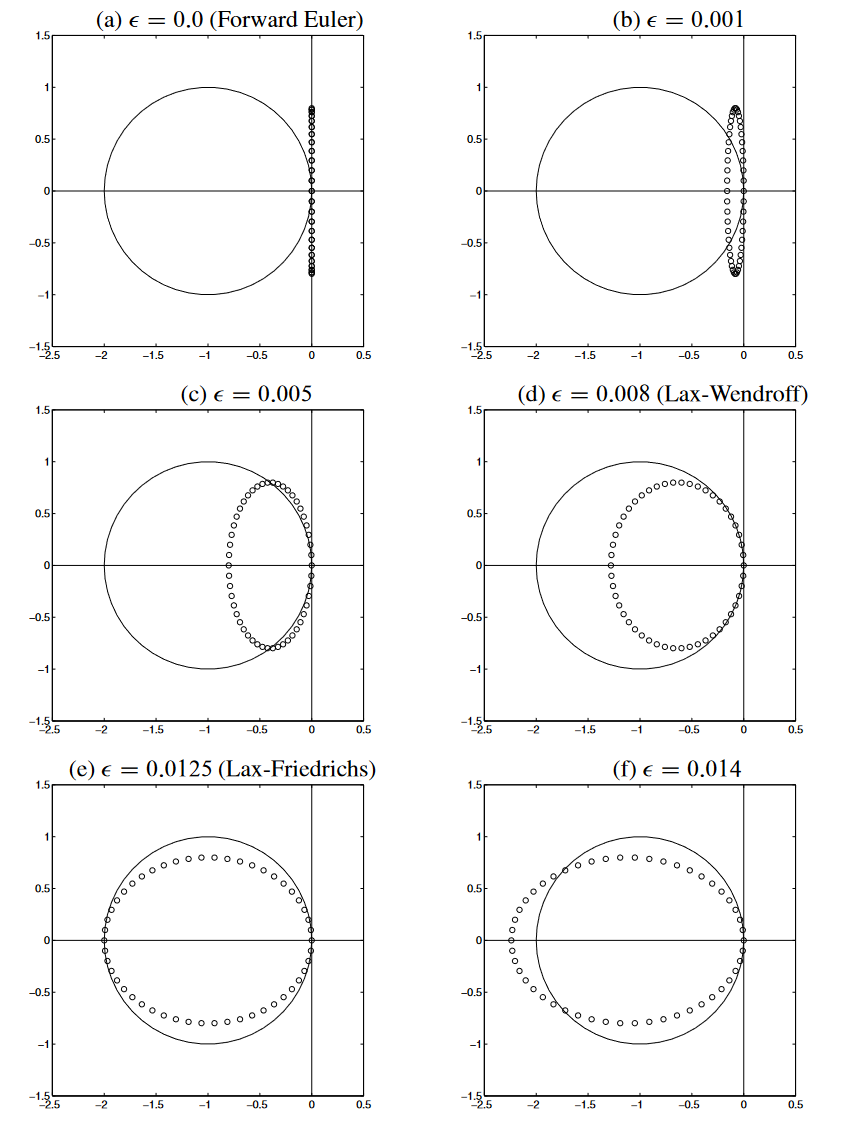
\includegraphics[width=0.8\textwidth]{figures/26-1.png}
    \label{fig 10.1}
    \caption{Eigenvalues of the matrix $A_\epsilon$ in , for various values of $\epsilon$, in the case $h=1 / 50$ and $k=0.8 h, a=1$, so ak/h=0.8. (a) shows the case $\epsilon=0$ which corresponds to the forward Euler method. (d) shows the case $\epsilon=a^2 k / 2$, the Lax-Wendroff method. (e) shows the case $\epsilon=h^2 / 2 k$, the Lax-Friedrichs method. The method is stable for $\epsilon$ between $a^2 k / 2$ and $h^2 / 2 k$, as in (d) through (e).}
\end{figure}
%────────────────────────────────────────